\documentclass{article}
\usepackage[a4paper]{geometry}
\usepackage{fancyhdr} 
\usepackage{tikz}
\usepackage{amsmath} 
\pagestyle{fancy}
\lhead{Abstände zwischen Punkten und Ebenen}
\rhead{Juli 2025}
\begin{document}
   
\newcommand{\norm}[1]{\big| {#1} \big|}  
\newcommand{\vect}[1]{\overrightarrow{#1}} 
\newcommand{\vectp}[1]{\vect{\mathrm{#1}}}
  
\section{Abstände zwischen Punkten und Ebenen}
 
\begin{minipage}[t]{\dimexpr\textwidth-5cm}
 Die einfachste Methode den Abstand zwischen einem Punkt und einer Ebene zu finden, ist das \emph{Lotfußpunktverfahren}. Dabei wird ein \emph{Lotfußpunkt} $\mathrm{F}$ bestimmt, welcher der zu $\mathrm{P}$ näheste, auf $\mathrm{E}$ liegende, Punkt ist. Die Länge des Verbindungsvektors $\vectp{PF}$ stellt nun den Abstand von $\mathrm{P}$ zu $\mathrm{E}$ dar. Somit ist der Abstand
 \[
  d(\mathrm{P}, \mathrm{E}) = \norm{\vectp{PF}}
 \] 
 Weil $\mathrm{F}$ in der Regel nicht in der Aufgabe gegeben ist, muss dieser Punkt erstmal gefunden werden. Dies wird getan, indem \\[-0.7em]
\end{minipage} 
\hfill
\begin{minipage}[t]{5cm}
 \centering 
 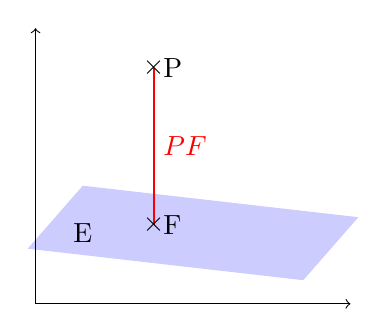
\begin{tikzpicture}[baseline=(current bounding box.north)] 
  \fill[blue!20] (-0.1, 0.7) -- (0.6, 1.5) -- (4.1,1.1) -- (3.4, 0.3) -- cycle;
  \draw (0.6, 0.9) node[black] {$\mathrm{E}$};
 
  \draw[thick,red] (1.5, 1) -- (1.5,3);
  \draw (1.5, 2) node[red, right] {$\vectp{PF}$}; 
  \draw (1.5, 3) node[black] {$\times$} node[right] {$\mathrm{P}$};  
  \draw (1.5, 1) node[black] {$\times$} node[right] {$\mathrm{F}$};
  \draw[->] (0, 0) -- (4, 0); 
  \draw[->] (0, 0) -- (0, 3.5);
 \end{tikzpicture}
\end{minipage}
eine Gerade, genannt die \emph{Lotgerade}, bestimmt wird, welche vom Punkt $\mathrm{P}$ aus auf direktestem Wege zur Ebene $\mathrm{E}$ geht. Offensichtlich muss die Lotgerade dafür Senkrecht zur Ebene sein, heißt kollinear zum Normalvektor $\vect{n}$. Daraus folgt die Lotgerade
\[
 g: \vect{x} = \vectp{OP} + t \cdot \vect{n} 
\]
Zusammen mit der Gleichung der Lotgerade und der Ebene kann nur deren Schnittpunkt, welcher auf der Lotfußpunkt $\mathrm{F}$ ist, gefunden werden, mithilfe dessen nun auch $\vectp{PF}$ und somit $\norm{\vectp{PF}}$ bestimmt werden kann.
 
Muss der Aufgabe nach $\mathrm{F}$ aber nicht angegeben werden, können die letzten wenigen Schritte aber auch übersprungen werden und 
\(
 d(\mathrm{P}, \mathrm{E}) = \norm{t} \cdot \norm{\vect{n}}
\)
genutzt werden. Dies folgt aus 
\begin{align*}
 d(\mathrm{P}, \mathrm{E}) &= \norm{\vectp{PF}} \\
  &= \norm{\vectp{OP} - \vectp{OF}} \\ 
  &= \norm{\vectp{OP} - (\vectp{OP} + t \cdot \vect{n})} \\
  &= \norm{t \cdot \vect{n}} \\
  &= \norm{t} \cdot \norm{\vect{n}}
\end{align*}
 
\subsection{Hesse'sche Normalform} 
 
\end{document}
 
